\documentclass[12pt]{article}

\usepackage[margin = .8in]{geometry}
\usepackage{amsmath}
\usepackage{graphicx}
\usepackage{multicol, enumerate}

\usepackage{fancyhdr}
\pagestyle{fancy}

\lhead{Math F113X: Numbers and Society}
\rhead{February 3, 2025}

\usepackage{tikz}
\usetikzlibrary{calc,trees,positioning,arrows,fit,shapes,calc}
\usetikzlibrary{patterns}
\usepackage{pgfplots}

\usepackage{longtable}
\usepackage{tabularx}

\newcommand{\ds}{\displaystyle}
\newcommand{\ans}[1][1in]{\rule{#1}{.5pt}}

\newcommand{\points}[1]{(#1 points.)}		% Trying to be lazy.

\usepackage{array}
\newcolumntype{L}[1]{>{\raggedright\let\newline\\\arraybackslash\hspace{0pt}}m{#1}}
\newcolumntype{C}[1]{>{\centering\let\newline\\\arraybackslash\hspace{0pt}}m{#1}}
\newcolumntype{R}[1]{>{\raggedleft\let\newline\\\arraybackslash\hspace{0pt}}m{#1}}
\newcommand{\red}[1]{\textcolor{red}{#1}}

%\topmargin -1in
%\textheight 9.5in
%\oddsidemargin -0.3in
%\evensidemargin \oddsidemargin
%\pagestyle{empty}
%%\marginparwidth 0.5in
%\textwidth 7in
%\parindent 0in

%--------------------------------------------------------------------------------------------------------------------------------------------------------------------------
%						Document
%--------------------------------------------------------------------------------------------------------------------------------------------------------------------------


\begin{document}
%\pagestyle{fancy}
\begin{center}
{\Large  Worksheet 6:  Fair Shares and Divider-Chooser 	}
\end{center}



\noindent \textbf{Group Names:} \hrulefill \\
%-------------------------------------------------------------------------------------------------------------
%						Assignment
%-----------------------------------------------------------------------------------------------------


%\begin{minipage}[b]{.6\linewidth}
Tom and Fred were given a cake worth \$12 that is equal parts strawberry, vanilla and chocolate.% Tom likes vanilla and strawberry the same but does not like chocolate at all. Fred will eat vanilla but likes strawberry twice as much as vanilla and likes chocolate three times as much as vanilla.

%\end{minipage}

\begin{center}
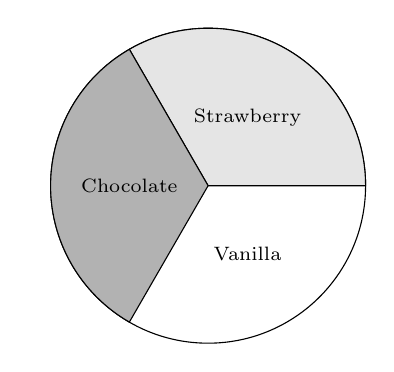
\begin{tikzpicture}
\def\r{2}
\draw (0,0) circle (\r cm);
\filldraw[fill= gray!20 ] (0,0) -- (0:\r) arc (0:120:\r) -- (0,0);
\path (60:1) node[]{{{\scriptsize Strawberry}}};
%\path node[right] (240:1) {{\scriptsize Strawberry}};
\filldraw[fill = gray!60 ] (0,0) -- (120:\r) arc (120:240:\r) -- (0,0);
\path (120+60:\r/2) node[]{{{\scriptsize Chocolate}}};
\path (-60:\r/2) node[]{{{\scriptsize Vanilla}}};
\end{tikzpicture}
\end{center}

%
%\begin{minipage}[b]{.4\linewidth}

%\end{minipage}

\begin{enumerate}
\item How much value is a fair share of the cake? \ans

\item Tom likes vanilla and strawberry equally, and doesn't like chocolate at all. 
\begin{enumerate}
\item How much does Tom value the vanilla section of the cake? \ans
\item How much does Tom value the chocolate section of the cake? \ans
\item How much does Tom value the strawberry section of the cake? \ans
\end{enumerate}
\hfill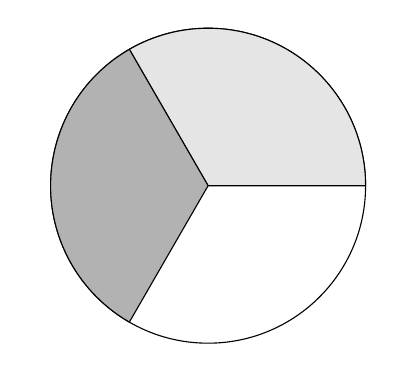
\begin{tikzpicture}
\draw (0,0) circle (2 cm);
\filldraw[fill= gray!20 ] (0,0) -- (0:2) arc (0:120:2) -- (0,0);
\filldraw[fill = gray!60 ] (0,0) -- (120:2) arc (120:240:2) -- (0,0);
\end{tikzpicture}

\item Fred will eat vanilla, but he likes strawberry twice as much as vanilla and he likes chocolate \emph{three} times as much as vanilla.
\begin{enumerate}
\item How much does Fred value the vanilla section of the cake? \ans
\item How much does Fred value the chocolate section of the cake? \ans
\item How much does Fred value the strawberry section of the cake? \ans
\end{enumerate}
\hfill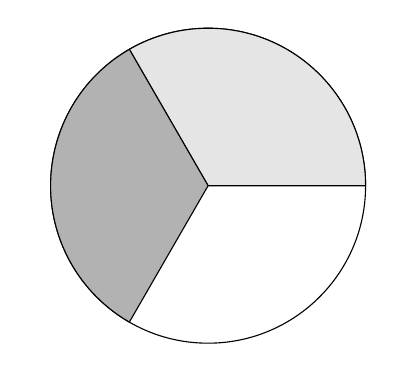
\begin{tikzpicture}
\draw (0,0) circle (2 cm);
\filldraw[fill= gray!20 ] (0,0) -- (0:2) arc (0:120:2) -- (0,0);
\filldraw[fill = gray!60 ] (0,0) -- (120:2) arc (120:240:2) -- (0,0);
\end{tikzpicture}

\newpage

For each of the following, assume you can subdivide the cake pieces as you like.

\item Find a way for Tom to divide the cake into two equal portions (they don't have to be connected) so that he values each portion equally. How does Fred value those two portions? Which one should he choose to get a fair share?
\def\r{1.2}

\begin{tikzpicture}
\draw (0,0) circle (\r cm);
\filldraw[fill= gray!20 ] (0,0) -- (0:\r) arc (0:120:\r) -- (0,0);
\filldraw[fill = gray!60 ] (0,0) -- (120:\r) arc (120:240:\r) -- (0,0);
\path (90:\r) node [above] {Tom's Values};
\end{tikzpicture}\hspace{2cm}\begin{tikzpicture}
\draw (0,0) circle (\r cm);
\filldraw[fill= gray!20 ] (0,0) -- (0:\r) arc (0:120:\r) -- (0,0);
\filldraw[fill = gray!60 ] (0,0) -- (120:\r) arc (120:240:\r) -- (0,0);
\path (90:\r) node [above] {Fred's Values};
\end{tikzpicture}
\vfill

Is it better to be the divider or chooser in this case? Why? 

\vspace{1cm}

\item Find two different ways for Fred to divide the cake into two shares (not necessarily connected) that he values equally. In each case, which share should Tom choose to make sure he gets his fair share?

\begin{tikzpicture}
\draw (0,0) circle (\r cm);
\filldraw[fill= gray!20 ] (0,0) -- (0:\r) arc (0:120:\r) -- (0,0);
\filldraw[fill = gray!60 ] (0,0) -- (120:\r) arc (120:240:\r) -- (0,0);
\path (90:\r) node [above] {Tom's Values};
\end{tikzpicture}\hspace{2cm}\begin{tikzpicture}
\draw (0,0) circle (\r cm);
\filldraw[fill= gray!20 ] (0,0) -- (0:\r) arc (0:120:\r) -- (0,0);
\filldraw[fill = gray!60 ] (0,0) -- (120:\r) arc (120:240:\r) -- (0,0);
\path (90:\r) node [above] {Fred's Values};
\end{tikzpicture}
\vfill

\begin{tikzpicture}
\draw (0,0) circle (\r cm);
\filldraw[fill= gray!20 ] (0,0) -- (0:\r) arc (0:120:\r) -- (0,0);
\filldraw[fill = gray!60 ] (0,0) -- (120:\r) arc (120:240:\r) -- (0,0);
\path (90:\r) node [above] {Tom's Values};
\end{tikzpicture}\hspace{2cm}\begin{tikzpicture}
\draw (0,0) circle (\r cm);
\filldraw[fill= gray!20 ] (0,0) -- (0:\r) arc (0:120:\r) -- (0,0);
\filldraw[fill = gray!60 ] (0,0) -- (120:\r) arc (120:240:\r) -- (0,0);
\path (90:\r) node [above] {Fred's Values};
\end{tikzpicture}
\vfill

Is it better to be the divider or chooser in this case? Why? 

\vspace{1cm}

\item Challenge: Suppose that another friend, Janet, likes vanilla 3 times as much as she likes strawberry and chocolate, which she likes equally. How much does she value each of the three pieces?

%\vspace{1.5in}
\hfill\begin{tikzpicture}
\draw (0,0) circle (\r cm);
\filldraw[fill= gray!20 ] (0,0) -- (0:\r) arc (0:120:\r) -- (0,0);
\filldraw[fill = gray!60 ] (0,0) -- (120:\r) arc (120:240:\r) -- (0,0);
\path (90:\r) node [above] {Janet's Values};
\end{tikzpicture}

Strawberry \ans Vanilla \ans Chocolate \ans

\end{enumerate}

\end{document}

%-------------------------------------------------------------------------------------------------------------------------------------------------------------------------------------------------------------------

%%% Local Variables:
%%% mode: latex
%%% TeX-master: t
%%% End:
